%%%%%%%%%%%%%%%%%%%%%%%%%%%%%%%%%%%%%%%%%%%%%%%%%%%%%%%%%%%
%				 _______ _    _  _____ 						
%				|__   __| |  | |/ ____|
%				   | |  | |__| | (___  
%				   | |  |  __  |\___ \ 
%				   | |  | |  | |____) |
%				   |_|  |_|  |_|_____/
%
%				 _               ____  
%				| |        /\   |  _ \ 
%				| |       /  \  | |_) |
%				| |      / /\ \ |  _ < 
%				| |____ / ____ \| |_) |
%				|______/_/    \_\____/ 
%
% _______ ______ __  __ _____  _            _______ ______ 
%|__   __|  ____|  \/  |  __ \| |        /\|__   __|  ____|
%   | |  | |__  | \  / | |__) | |       /  \  | |  | |__   
%   | |  |  __| | |\/| |  ___/| |      / /\ \ | |  |  __|  
%   | |  | |____| |  | | |    | |____ / ____ \| |  | |____ 
%   |_|  |______|_|  |_|_|    |______/_/    \_\_|  |______|
%
%%%%%%%%%%%%%%%%%%%%%%%%%%%%%%%%%%%%%%%%%%%%%%%%%%%%%%%%%%%
%%%%%%%%%%%%%%%%%%%%%%%%%%%%%%%%%%%%%%%%%%%%%%%%%%%%%%%%%%%
%%%%% DONT CHANGE ANYTHING BEFORE THE "TITLE" SECTION.%%%%%
%%%%%%%%%%%%%%%%%%%%%%%%%%%%%%%%%%%%%%%%%%%%%%%%%%%%%%%%%%%
%%%%%%%%%%%%%%%%%%%%%%%%%%%%%%%%%%%%%%%%%%%%%%%%%%%%%%%%%%%
\documentclass{article} % Don't change this
% _____        _____ _  __          _____ ______  _____ 
%|  __ \ /\   / ____| |/ /    /\   / ____|  ____|/ ____|
%| |__) /  \ | |    | ' /    /  \ | |  __| |__  | (___  
%|  ___/ /\ \| |    |  <    / /\ \| | |_ |  __|  \___ \ 
%| |  / ____ \ |____| . \  / ____ \ |__| | |____ ____) |
%|_| /_/    \_\_____|_|\_\/_/    \_\_____|______|_____/ 
%%%%%%%%%%%%%%%%%%%%%%%%%%%%%%%%%%%%%%%%%%%%%%%%%%%%%%%%

\usepackage[english]{babel}
\usepackage[utf8]{inputenc}
\usepackage[margin=1in]{geometry}
\usepackage{amsmath}
\usepackage{amsthm}
\usepackage{amsfonts}
\usepackage{amssymb}
\usepackage[usenames,dvipsnames]{xcolor}
\usepackage{graphicx}
\usepackage[siunitx]{circuitikz}
\usepackage{tikz}
\usepackage[colorinlistoftodos, color=orange!50]{todonotes}
\usepackage{hyperref}
\usepackage[numbers, square]{natbib}
\usepackage{fancybox}
\usepackage{epsfig}
\usepackage{soul}
\usepackage[framemethod=tikz]{mdframed}


\usepackage{algorithm}
\usepackage[noend]{algpseudocode}

\usepackage[T1]{fontenc}
\usepackage[utf8]{inputenc}

%%%%%%%%%%%%%%%%%%%%%%%%%%%%%%%%%%%%%%%%%%%%%%%%%%%%%%%


%	  _____ _    _  _____ _______ ____  __  __ 
%	 / ____| |  | |/ ____|__   __/ __ \|  \/  |
%	| |    | |  | | (___    | | | |  | | \  / |
%	| |    | |  | |\___ \   | | | |  | | |\/| |
%	| |____| |__| |____) |  | | | |__| | |  | |
%	 \_____|\____/|_____/   |_|  \____/|_|  |_|
%%%%%%%%%%%%%%%%%%%%%%%%%%%%%%%%%%%%%%%%%%%%%%%%
%  _____ ____  __  __ __  __          _   _ _____   _____ 
% / ____/ __ \|  \/  |  \/  |   /\   | \ | |  __ \ / ____|
%| |   | |  | | \  / | \  / |  /  \  |  \| | |  | | (___  
%| |   | |  | | |\/| | |\/| | / /\ \ | . ` | |  | |\___ \ 
%| |___| |__| | |  | | |  | |/ ____ \| |\  | |__| |____) |
% \_____\____/|_|  |_|_|  |_/_/    \_\_| \_|_____/|_____/ 
%%%%%%%%%%%%%%%%%%%%%%%%%%%%%%%%%%%%%%%%%%%%%%%%%%%%%%%%%%

% SYNTAX FOR NEW COMMANDS:
%\newcommand{\new}{Old command or text}

% EXAMPLE:

\newcommand{\blah}{blah blah blah \dots}
\newcommand{\subf}[2]{%
  {\small\begin{tabular}[t]{@{}c@{}}
  #1\\#2
  \end{tabular}}%
}
%%%%%%%%%%%%%%%%%%%%%%%%%%%%%%%%%%%%%%%%%%%%%%%%%%%%%%%%%
%  _______ ______          _____ _    _ ______ _____  
% |__   __|  ____|   /\   / ____| |  | |  ____|  __ \ 
%    | |  | |__     /  \ | |    | |__| | |__  | |__) |
%    | |  |  __|   / /\ \| |    |  __  |  __| |  _  / 
%    | |  | |____ / ____ \ |____| |  | | |____| | \ \ 
%    |_|  |______/_/    \_\_____|_|  |_|______|_|  \_\
%%%%%%%%%%%%%%%%%%%%%%%%%%%%%%%%%%%%%%%%%%%%%%%%%%%%%%%%%
% \english
% \units 
% \spelling 
% \source 
% \concept
% \arbitrary{comment}{points}
% \summary{General Comments}

\setlength{\marginparwidth}{1cm}

% NEW COUNTERS
\newcounter{points}
\setcounter{points}{100}
\newcounter{spelling}
\newcounter{usage}
\newcounter{units}
\newcounter{other}
\newcounter{source}
\newcounter{concept}
\newcounter{missing}
\newcounter{math}

% COMMANDS
%\newcommand{\raisa}[2]{\colorbox{Yellow}{#1} \todo{#2}}
\newcommand{\arbitrary}[2]{\todo{#1 #2} \addtocounter{points}{#2} \addtocounter{other}{#2}}
\newcommand{\english}{\todo{LANGUAGE (-1)} \addtocounter{points}{-1}
\addtocounter{usage}{-1}}
\newcommand{\units}{\todo{UNITS (-1)} \addtocounter{points}{-1}
\addtocounter{units}{-1}}
\newcommand{\spelling}{\todo{SPELLING and GRAMMAR (-1)} \addtocounter{points}{-1}
\addtocounter{spelling}{-1}}
\newcommand{\source}{\todo{SOURCE(S) (-2)} \addtocounter{points}{-2}
\addtocounter{source}{-2}}
\newcommand{\concept}{\todo{CONCEPT (-2)} \addtocounter{points}{-2}
\addtocounter{concept}{-2}}
\newcommand{\missing}[2]{\todo{MISSING CONTENT (#1) #2} \addtocounter{points}{#1}
\addtocounter{missing}{#1}}
\newcommand{\maths}{\todo{MATH (-1)} \addtocounter{points}{-1}
\addtocounter{math}{-1}}

\newcommand{\summary}[1]{
\begin{mdframed}[nobreak=true]
\begin{minipage}{\textwidth}
\vspace{0.5cm}
\begin{center}
\Large{Grade Summary} \hrule 
\end{center} \vspace{0.5cm}
General Comments: #1

% \vspace{0.5cm}
Possible Points \dotfill 100 \\
Points Lost (Spelling and Grammar) \dotfill \thespelling \\
Points Lost (Language) \dotfill \theusage \\
Points Lost (Units) \dotfill \theunits \\
Points Lost (Math) \dotfill \themath \\
Points Lost (Sources) \dotfill \thesource \\
Points Lost (Concept) \dotfill \theconcept \\
Points Lost (Missing Content) \dotfill \themissing \\
Other \dotfill \theother \\[0.5cm]
\begin{center}
\large{\textbf{Grade:} \fbox{\thepoints}}
\end{center}
\end{minipage}
\end{mdframed}}

%#########################################################

%To use symbols for footnotes
\renewcommand*{\thefootnote}{\fnsymbol{footnote}}
%To change footnotes back to numbers uncomment the following line
%\renewcommand*{\thefootnote}{\arabic{footnote}}

% Enable this command to adjust line spacing for inline math equations.
% \everymath{\displaystyle}

% _______ _____ _______ _      ______ 
%|__   __|_   _|__   __| |    |  ____|
%   | |    | |    | |  | |    | |__   
%   | |    | |    | |  | |    |  __|  
%   | |   _| |_   | |  | |____| |____ 
%   |_|  |_____|  |_|  |______|______|
%%%%%%%%%%%%%%%%%%%%%%%%%%%%%%%%%%%%%%%

\title{
\normalfont \normalsize 
\textsc{Computational Neuroscience \\ 
IIT Madras} \\
[10pt] 
\rule{\linewidth}{0.5pt} \\[6pt] 
\huge Assignment 3 : Convolutional Neural Network \\
\rule{\linewidth}{2pt}  \\[10pt]
}
\author{Ganga Meghanath \\
EE15B025}

\begin{document}

\maketitle
% \noindent
% Date Performed \dotfill January 0, 0000 \\
% Partners \dotfill Full Name \\
% Instructor \dotfill Full Name \\

%%%%%%%%%%%%%%%%%%%%%%%%%%%%%%%%%%%%%%%

%			  ______      ____  
%			 |  ____/\   / __ \ 
%			 | |__ /  \ | |  | |
%			 |  __/ /\ \| |  | |
%			 | | / ____ \ |__| |
%			 |_|/_/    \_\___\_\
%%%%%%%%%%%%%%%%%%%%%%%%%%%%%%%%%%%%%%%%

%
% Ctrl + / to comment out a group of lines.
%
%
% LIST MORE COMMON COMMMANDS
% LIST USEFUL WEBSITES FOR TABLES, ETC
% WHAT TO DO WHEN YOUR CODE WONT COMPILE
% OVERLEAF SHORTCUTS
%



%%%%%%%%%%%%%%%%%%%%%%%%%%%%%%%%%%%%%%%


% _               ____  
%| |        /\   |  _ \ 
%| |       /  \  | |_) |
%| |      / /\ \ |  _ < 
%| |____ / ____ \| |_) |
%|______/_/    \_\____/ 
%%%%%%%%%%%%%%%%%%%%%%%%
%  _____ _______       _____ _______ _____ 
% / ____|__   __|/\   |  __ \__   __/ ____|
%| (___    | |  /  \  | |__) | | | | (___  
% \___ \   | | / /\ \ |  _  /  | |  \___ \ 
% ____) |  | |/ ____ \| | \ \  | |  ____) |
%|_____/   |_/_/    \_\_|  \_\ |_| |_____/ 
%%%%%%%%%%%%%%%%%%%%%%%%%%%%%%%%%%%%%%%%%%%
% _    _ ______ _____  ______ 
%| |  | |  ____|  __ \|  ____|
%| |__| | |__  | |__) | |__   
%|  __  |  __| |  _  /|  __|  
%| |  | | |____| | \ \| |____ 
%|_|  |_|______|_|  \_\______|
%%%%%%%%%%%%%%%%%%%%%%%%%%%%%%
\section{Aim}

Understanding convolutional neural networks

\section{Dataset Analysis}
The dataset comprises of handwritten digits ranging from 0 to 9 as shown below (color and grayscale):

\begin{figure}[H]
\begin{tabular}{ccccc}
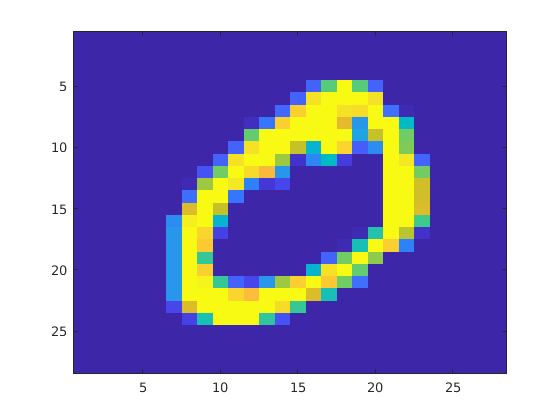
\includegraphics[width=0.15\linewidth]{images/0.png}
&
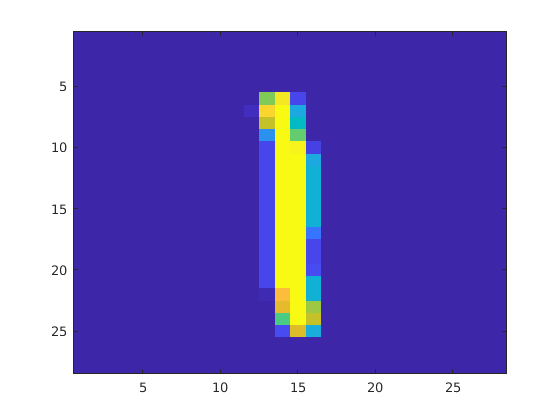
\includegraphics[width=0.15\linewidth]{images/1.png}
&
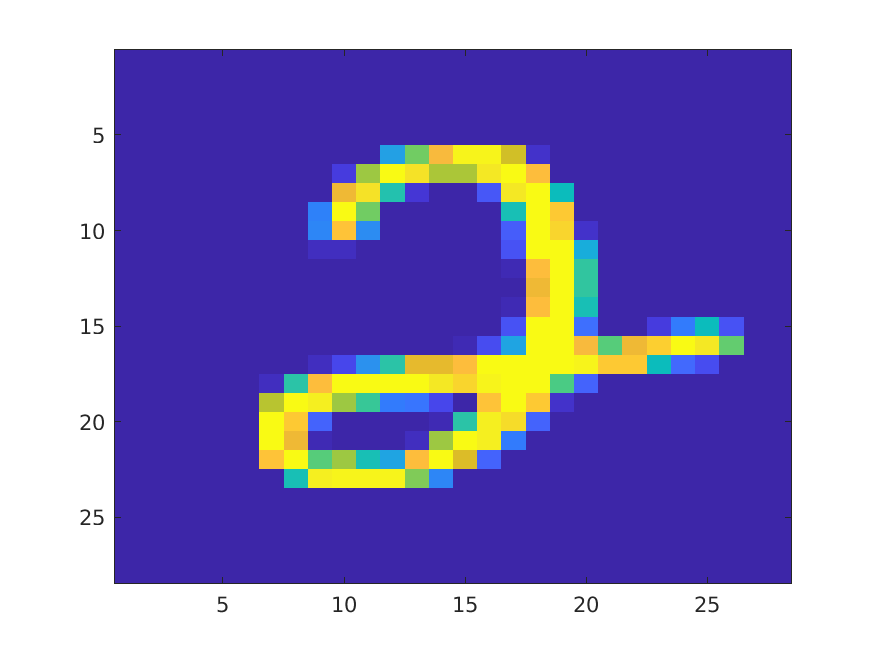
\includegraphics[width=0.15\linewidth]{images/2.png}
&
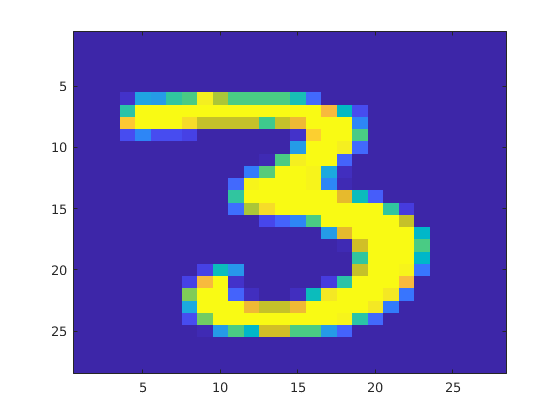
\includegraphics[width=0.15\linewidth]{images/3.png}
&
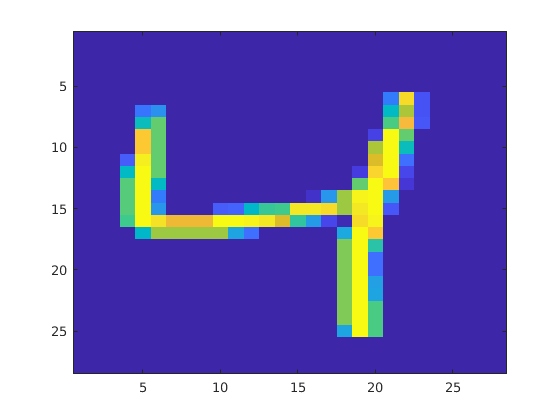
\includegraphics[width=0.15\linewidth]{images/4.png}
\\
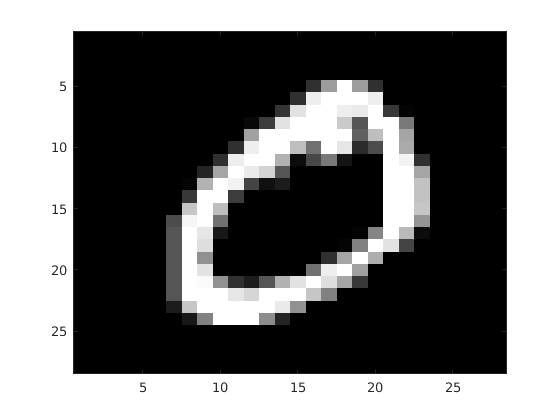
\includegraphics[width=0.15\linewidth]{images/0_gray.png}
&
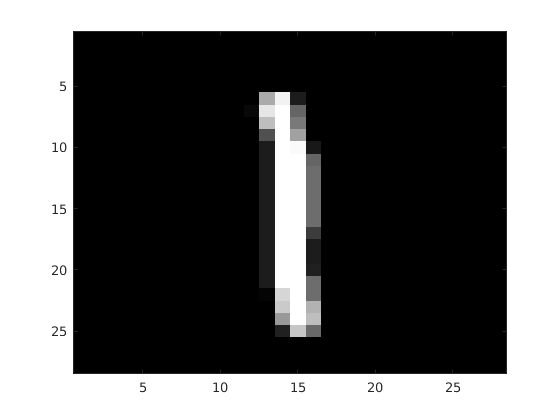
\includegraphics[width=0.15\linewidth]{images/1_gray.png}
&
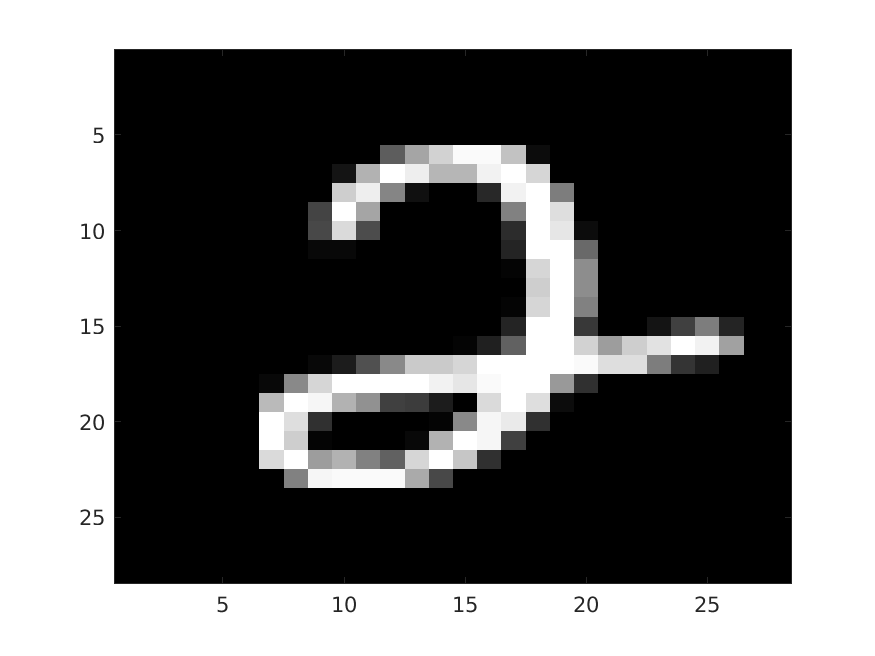
\includegraphics[width=0.15\linewidth]{images/2_gray.png}
&
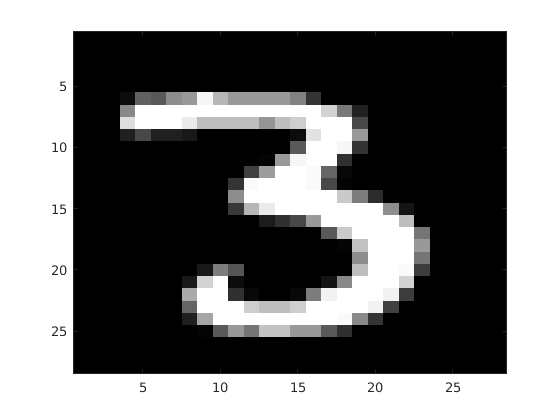
\includegraphics[width=0.15\linewidth]{images/3_gray.png}
&
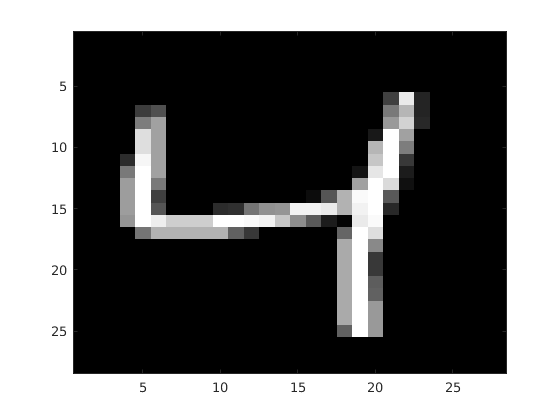
\includegraphics[width=0.15\linewidth]{images/4_gray.png}
\\
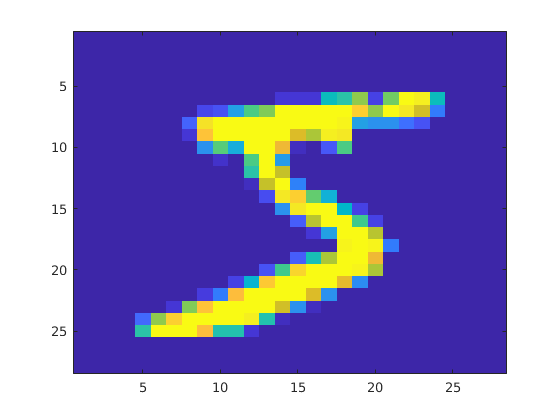
\includegraphics[width=0.15\linewidth]{images/5.png}
&
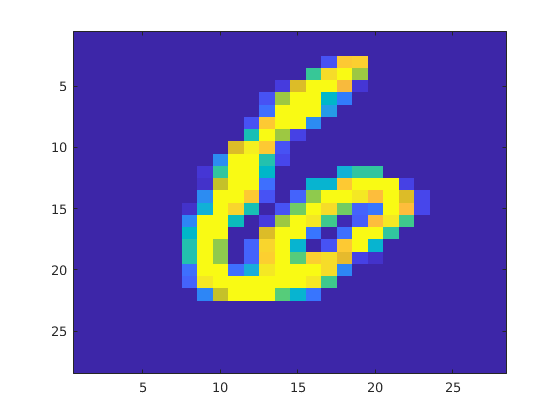
\includegraphics[width=0.15\linewidth]{images/6.png}
&
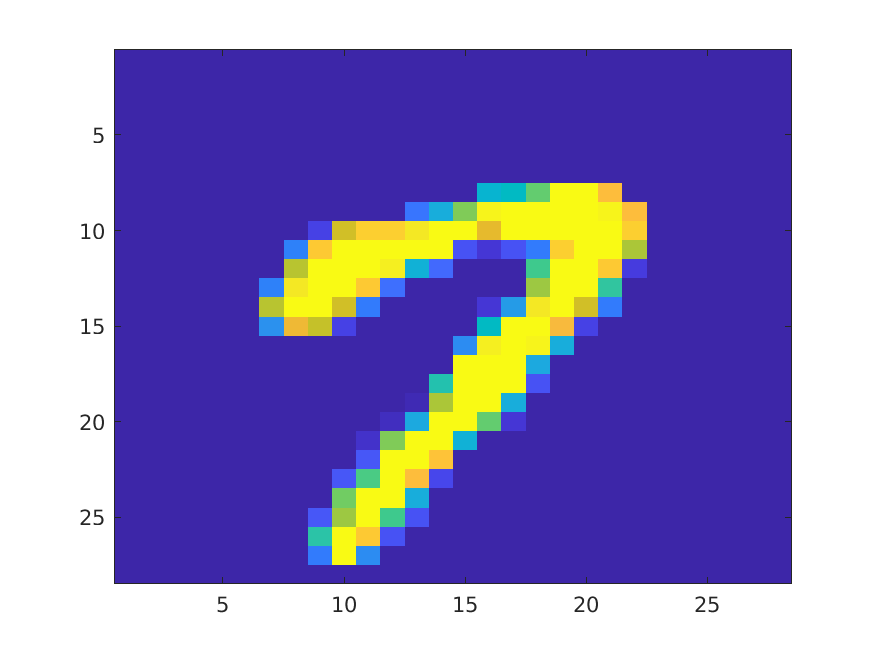
\includegraphics[width=0.15\linewidth]{images/7.png}
&
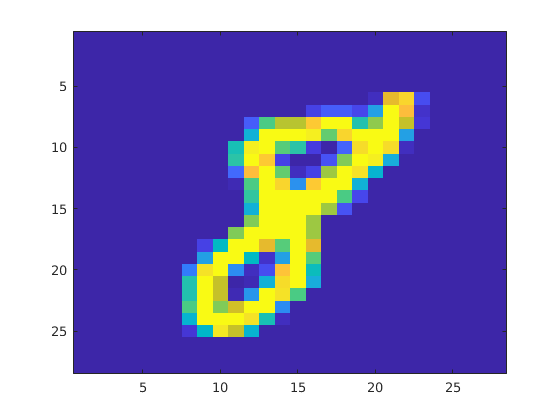
\includegraphics[width=0.15\linewidth]{images/8.png}
&
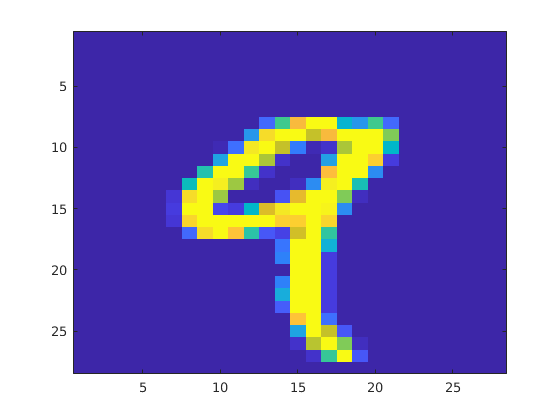
\includegraphics[width=0.15\linewidth]{images/9.png}
\\
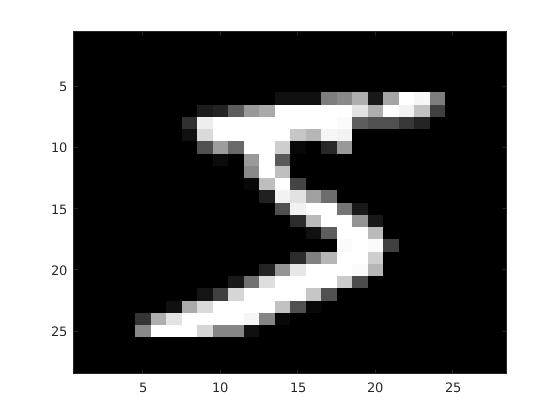
\includegraphics[width=0.15\linewidth]{images/5_gray.png}
&
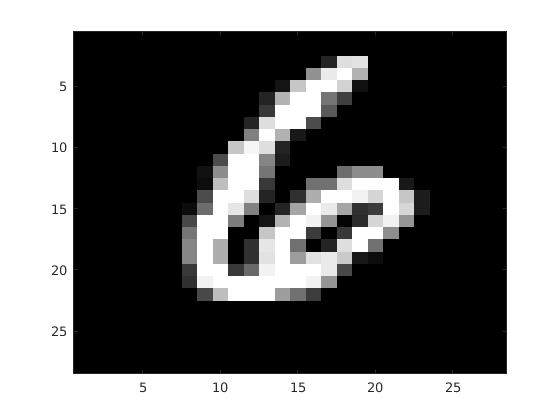
\includegraphics[width=0.15\linewidth]{images/6_gray.png}
&
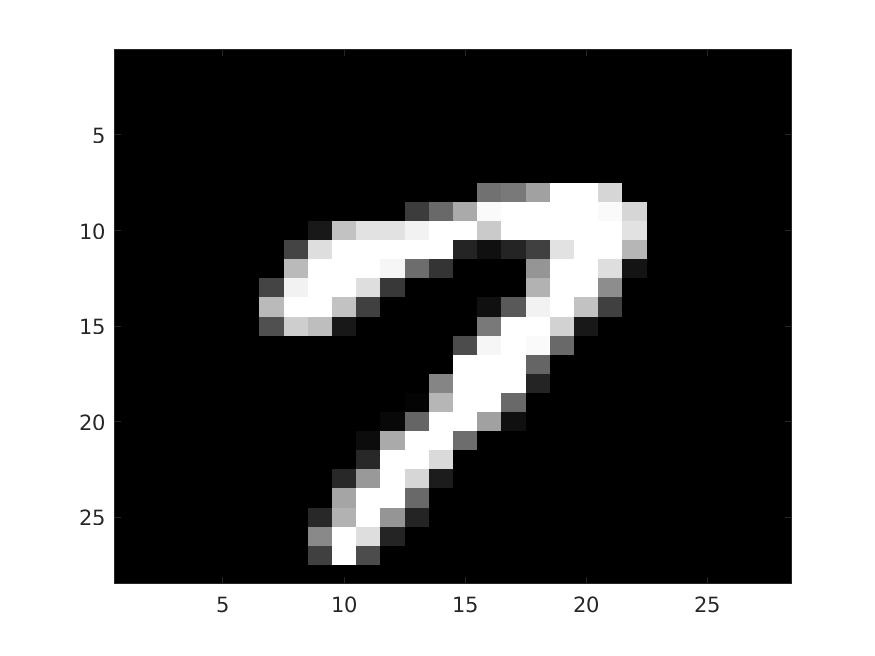
\includegraphics[width=0.15\linewidth]{images/7_gray.png}
&
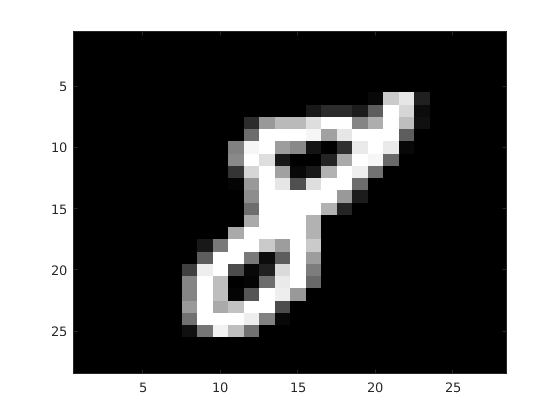
\includegraphics[width=0.15\linewidth]{images/8_gray.png}
&
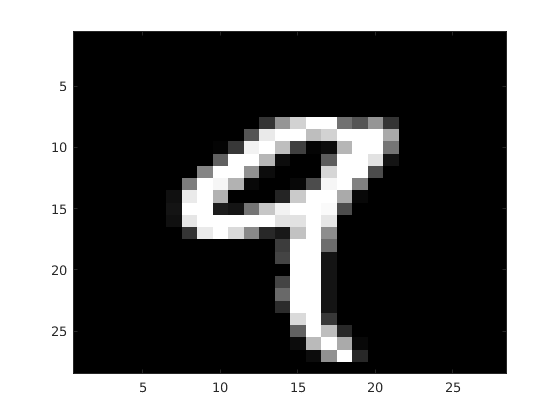
\includegraphics[width=0.15\linewidth]{images/9_gray.png}
\end{tabular}
\end{figure}

The dataset has been visualised using : \\
$$ \textrm{figure(1);imagesc(images(:,:,i));} $$
$$ \textrm{figure(2);imagesc(images(:,:,i));colormap(gray);} $$
where i stands for the $i^{th}$ datapoint in the training set.

%%%%%%%%%%%%%%%%%%%%%%%%%%%%%%%%%%%%%%%%%%%%%%%%%%%%%%%%%%%%%%%%%
\section{Question 1}
%------------------------------------------------------
\subsection{Performance}
The performance after training using the given configuration is :
\begin{table}[H]
  \begin{center}
    \begin{tabular}{|c|c|c|c|} % <-- Alignments: 1st column left, 2nd middle and 3rd right, with vertical lines in between
    \hline
      \textbf{No. of Epochs} & \textbf{No. of Filters} & \textbf{Filter size} & \textbf{No. of training data}\\
      \hline
      3 & 20 & 9 & 10000 \\
      \hline
    \end{tabular}
  \end{center}
\end{table}

\begin{table}[H]
  \begin{center}
    \begin{tabular}{|c|c|c|} % <-- Alignments: 1st column left, 2nd middle and 3rd right, with vertical lines in between
    \hline
      \textbf{Training time} & \textbf{No. of test images} & \textbf{Accuracy}\\
      \hline
      141.47s & 10000 & 93.14$\%$ \\
      \hline
    \end{tabular}
  \end{center}
\end{table}

Note : The CNN$\_$Network has been saved.

%%%%%%%%%%%%%%%%%%%%%%%%%%%%%%%%%%%%%%%%%%%%%%%%%%%%%%%%%%%%%%%%%
\newpage
\section{Question 2}

The visualisation of the weights for :
\begin{table}[H]
  \begin{center}
    \begin{tabular}{|c|c|c|c|} % <-- Alignments: 1st column left, 2nd middle and 3rd right, with vertical lines in between
    \hline
      \textbf{No. of Epochs} & \textbf{No. of Filters} & \textbf{Filter size} & \textbf{No. of training data}\\
      \hline
      3 & 20 & 9 & 10000 \\
      \hline
    \end{tabular}
  \end{center}
\end{table}

has been portrayed below. Note that the edges are more easily identifyable in the grayscaled version of the filter plots.

\begin{figure}[H]
\centering
\begin{tabular}{cccc}
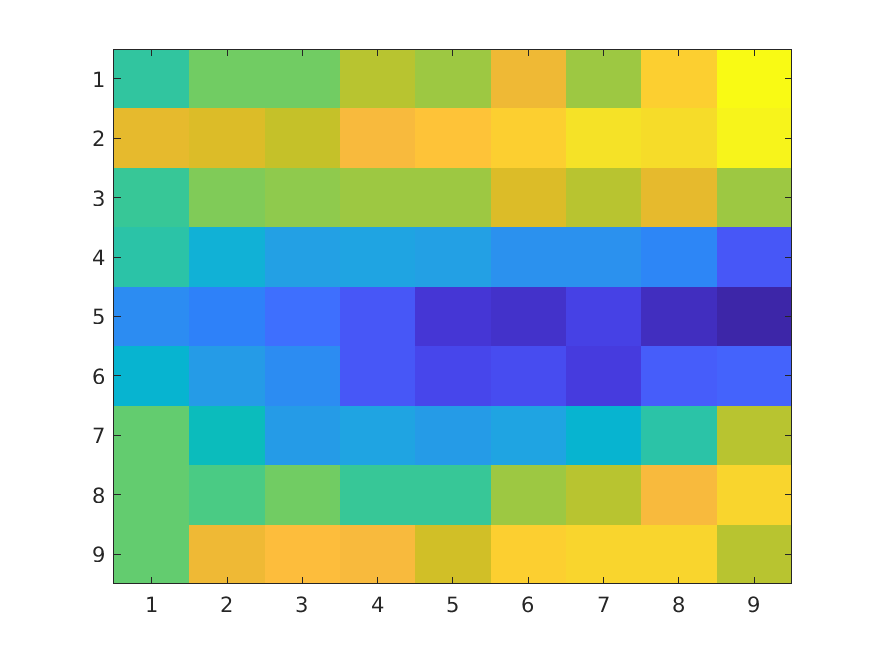
\includegraphics[width=0.2\linewidth]{images/Fig_weights_1.png}
&
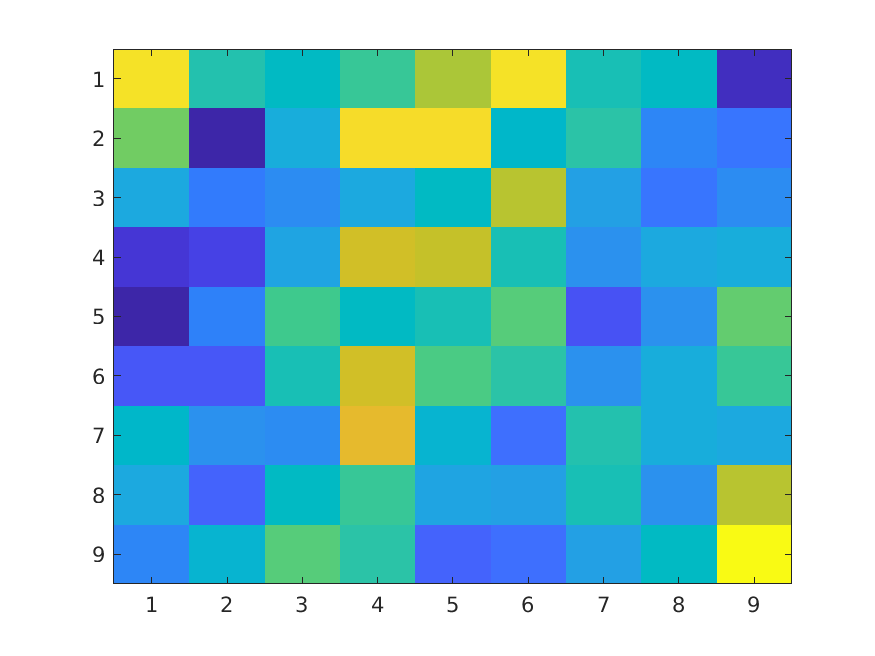
\includegraphics[width=0.2\linewidth]{images/Fig_weights_2.png}
&
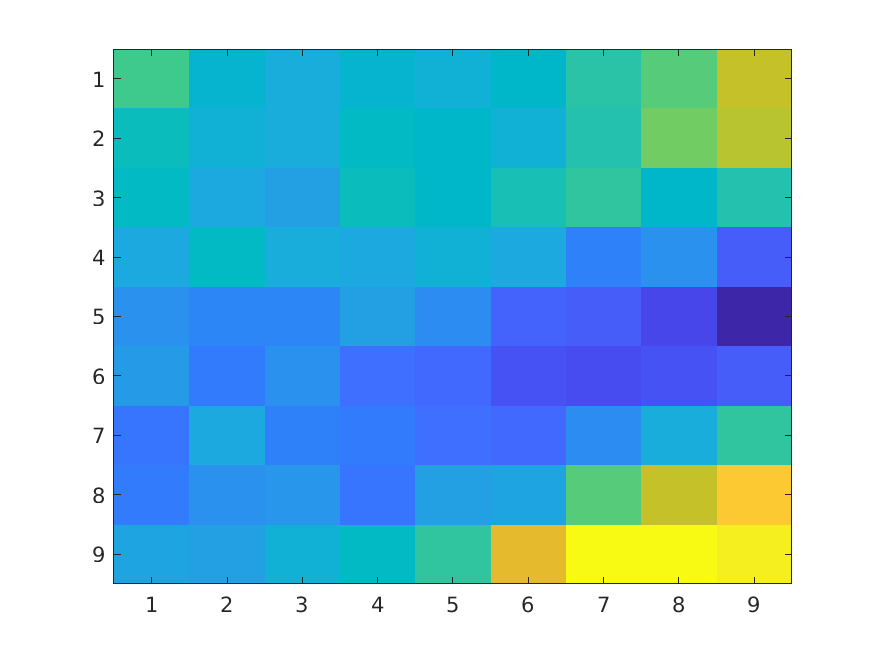
\includegraphics[width=0.2\linewidth]{images/Fig_weights_3.png}
&
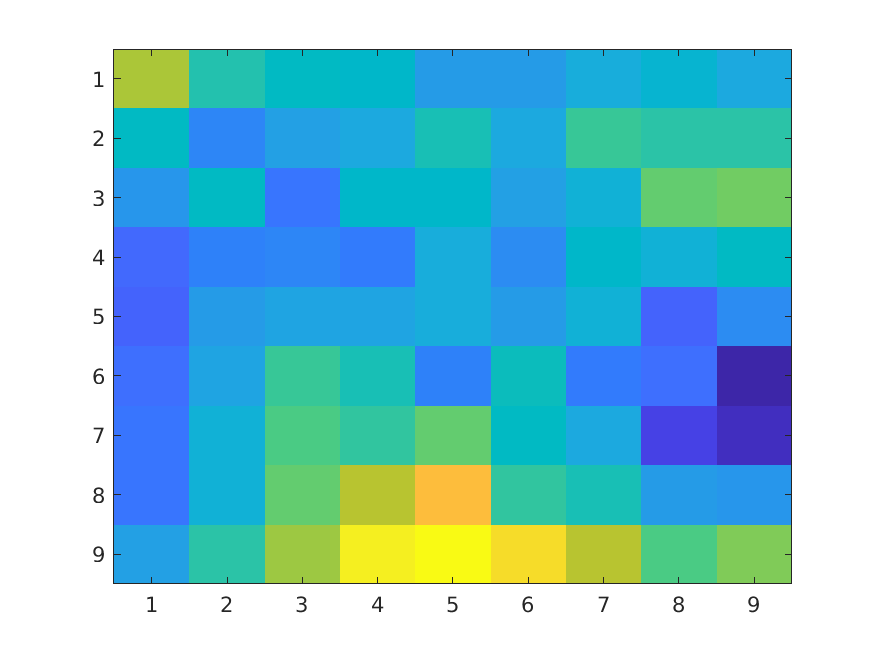
\includegraphics[width=0.2\linewidth]{images/Fig_weights_4.png}
\\
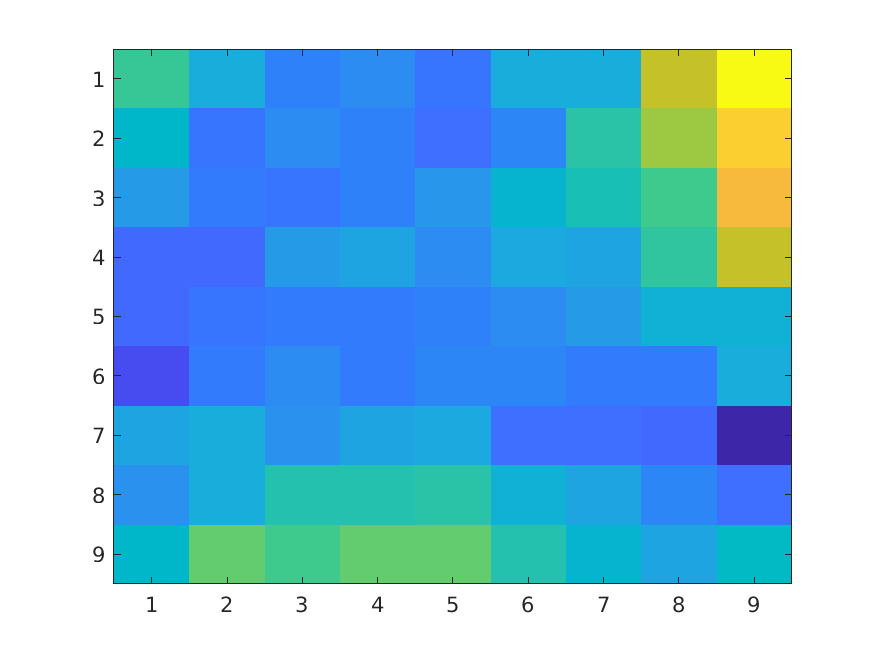
\includegraphics[width=0.2\linewidth]{images/Fig_weights_5.png}
&
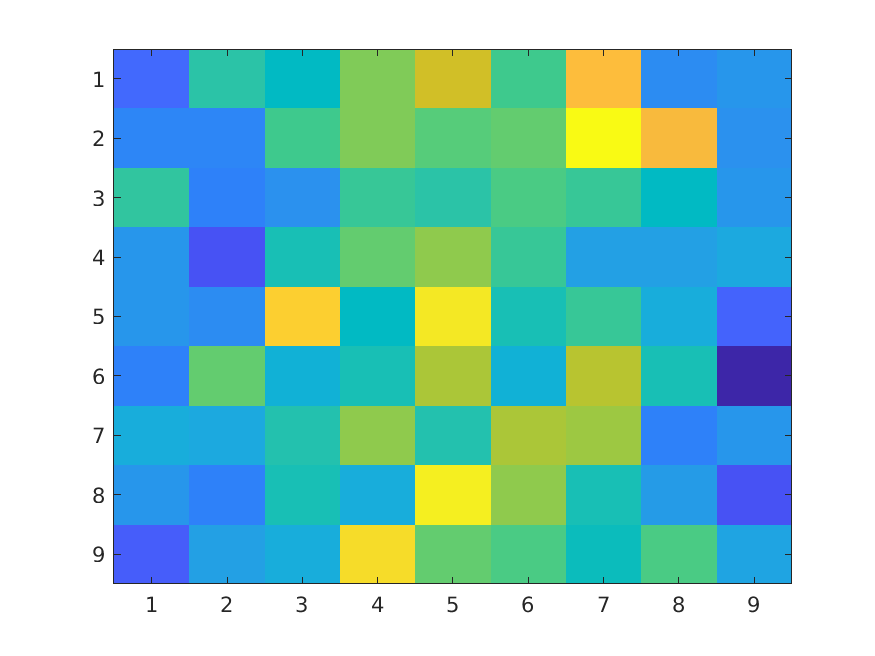
\includegraphics[width=0.2\linewidth]{images/Fig_weights_6.png}
&
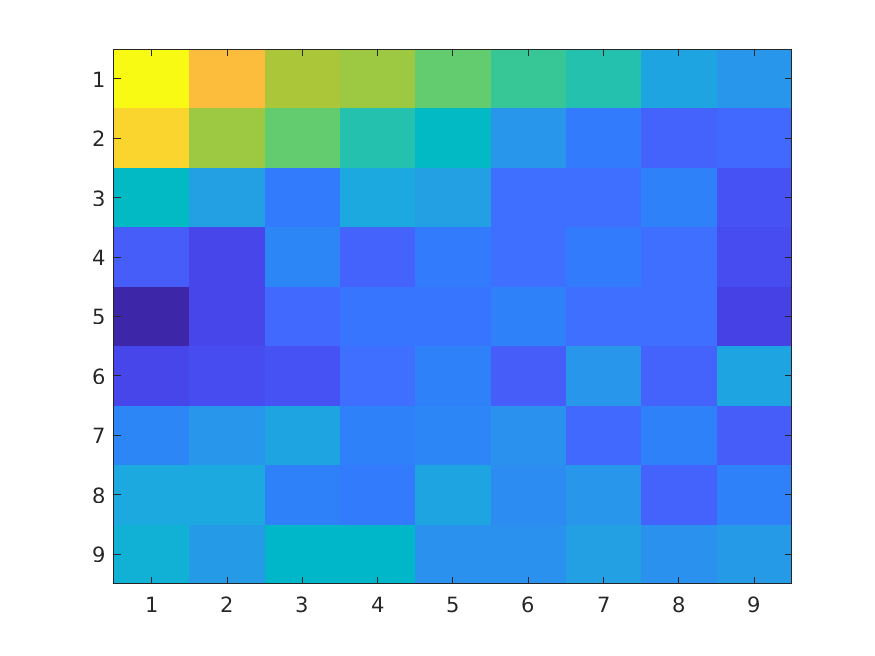
\includegraphics[width=0.2\linewidth]{images/Fig_weights_7.png}
&
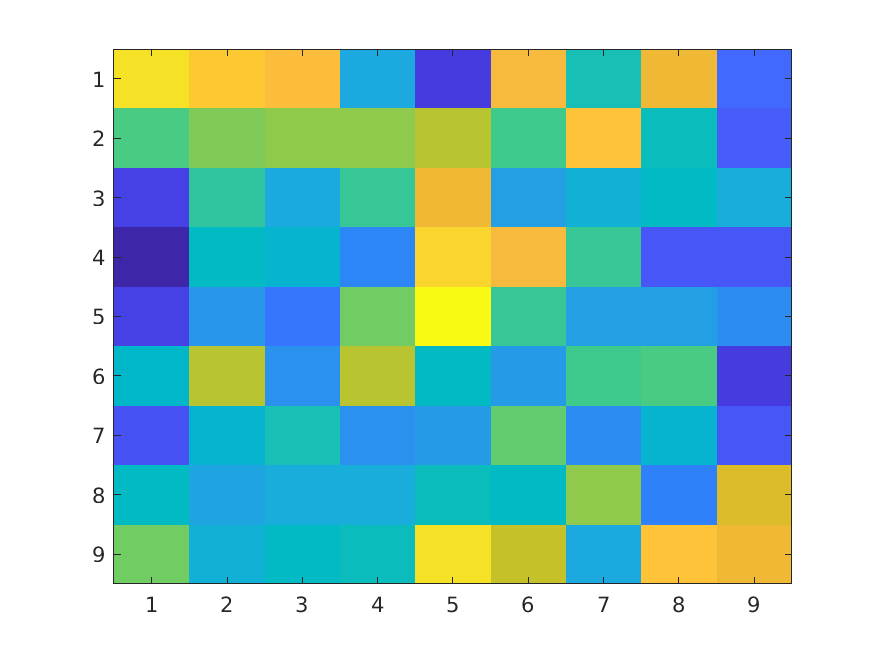
\includegraphics[width=0.2\linewidth]{images/Fig_weights_8.png}
\\
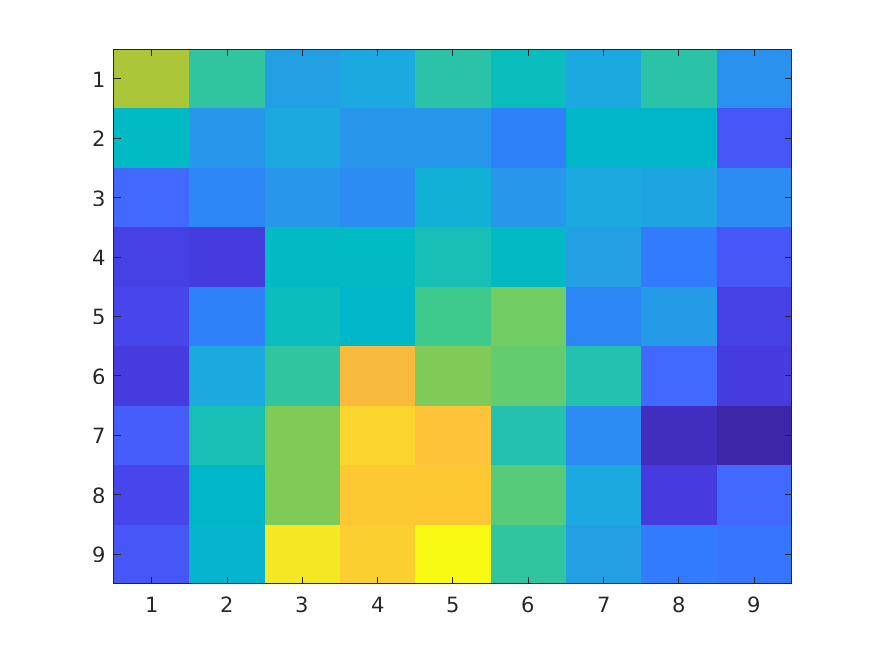
\includegraphics[width=0.2\linewidth]{images/Fig_weights_9.png}
&
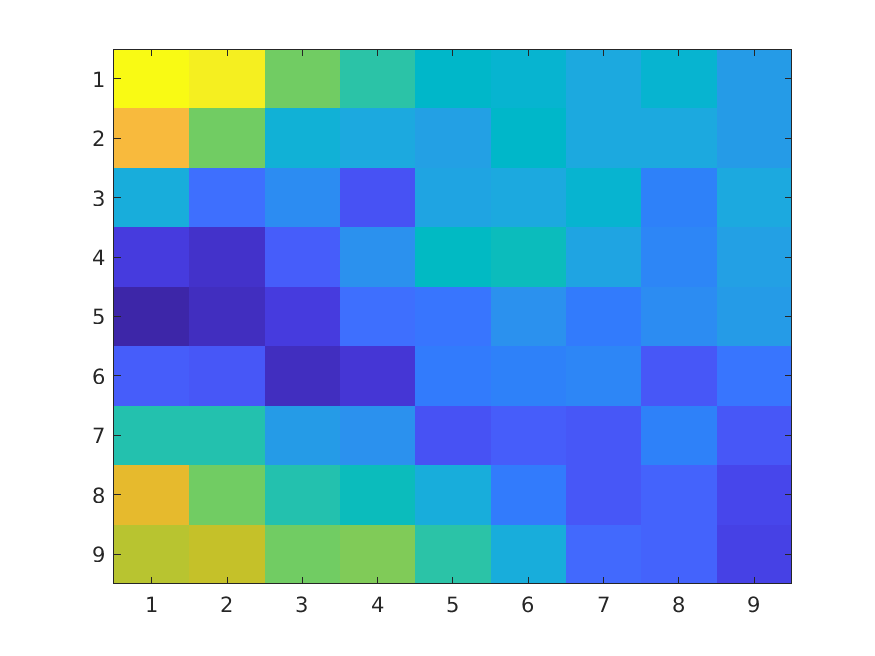
\includegraphics[width=0.2\linewidth]{images/Fig_weights_10.png}
&
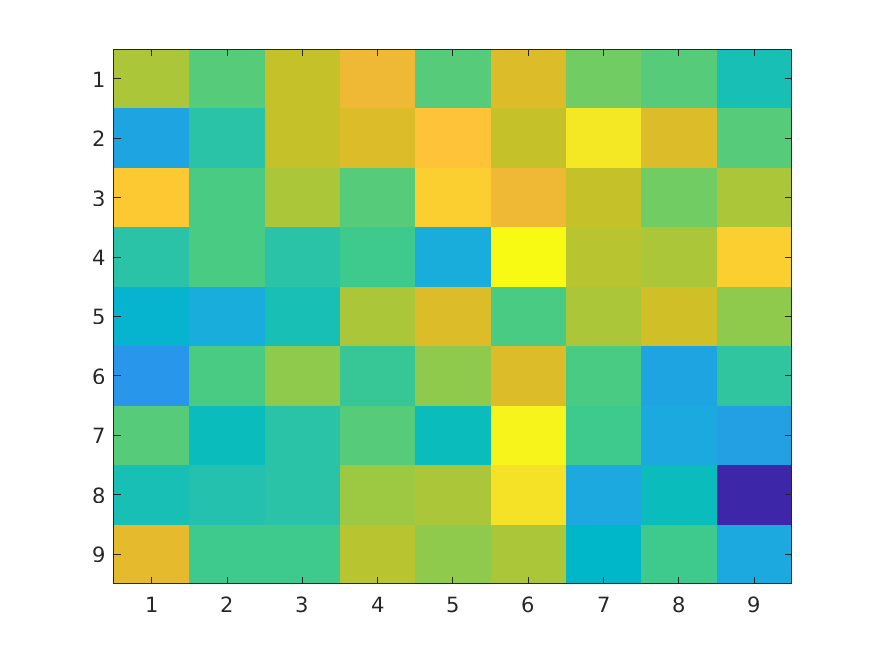
\includegraphics[width=0.2\linewidth]{images/Fig_weights_11.png}
&
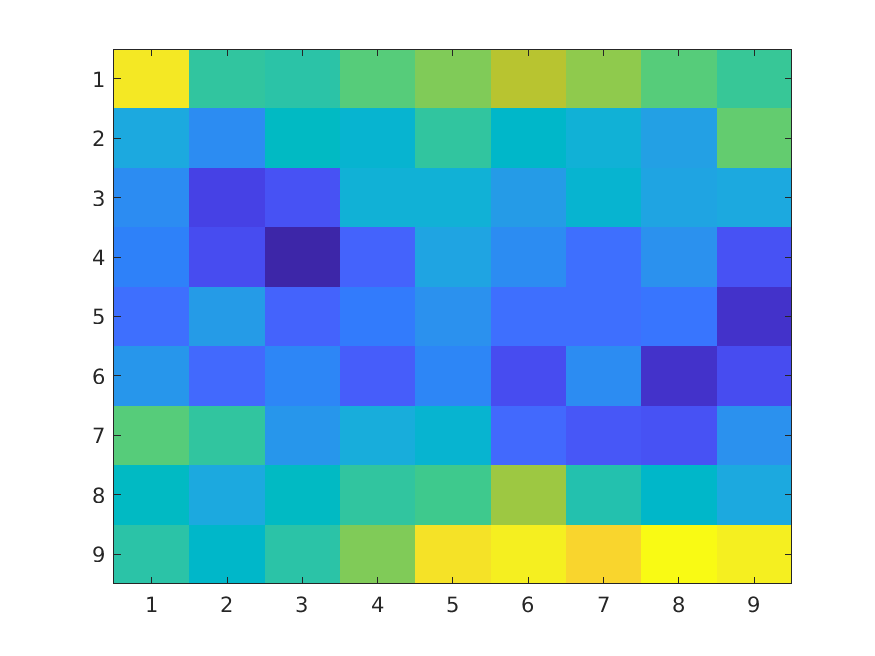
\includegraphics[width=0.2\linewidth]{images/Fig_weights_12.png}
\\
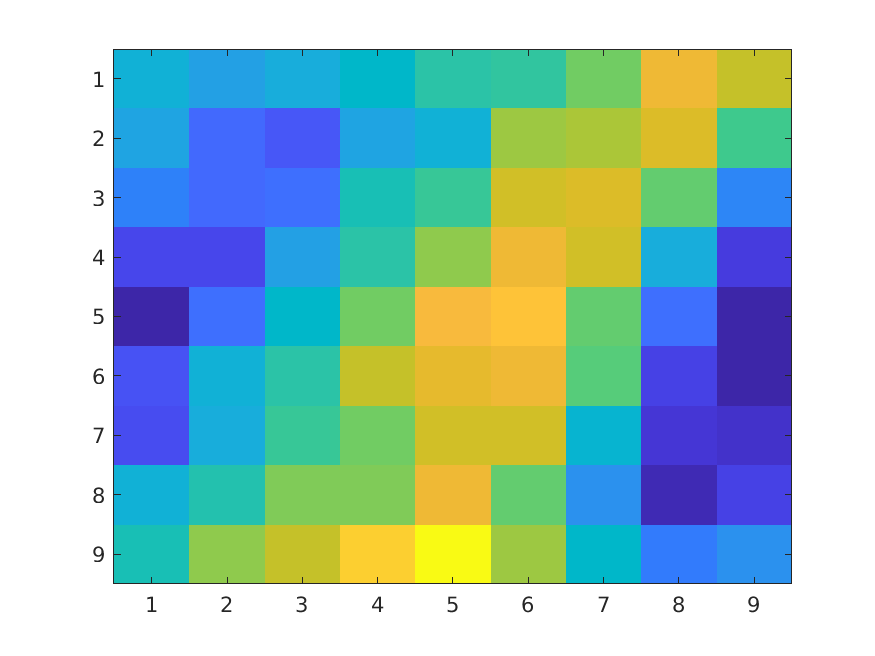
\includegraphics[width=0.2\linewidth]{images/Fig_weights_13.png}
&
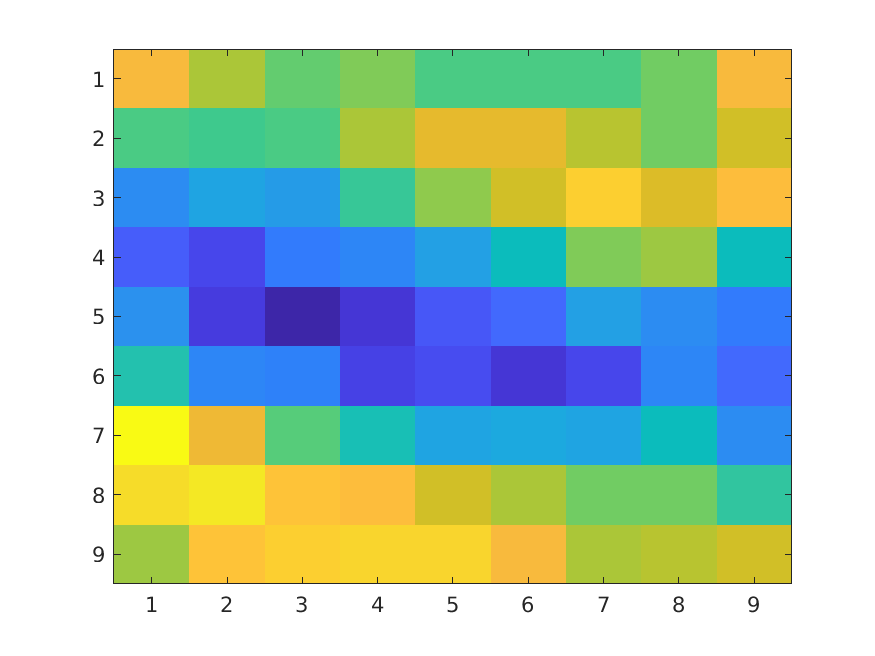
\includegraphics[width=0.2\linewidth]{images/Fig_weights_14.png}
&
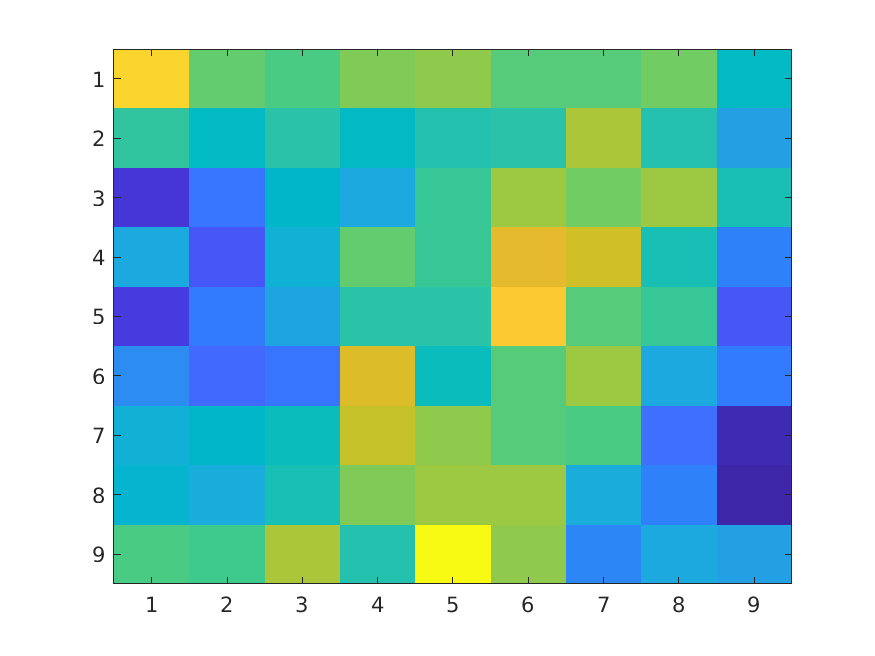
\includegraphics[width=0.2\linewidth]{images/Fig_weights_15.png}
&
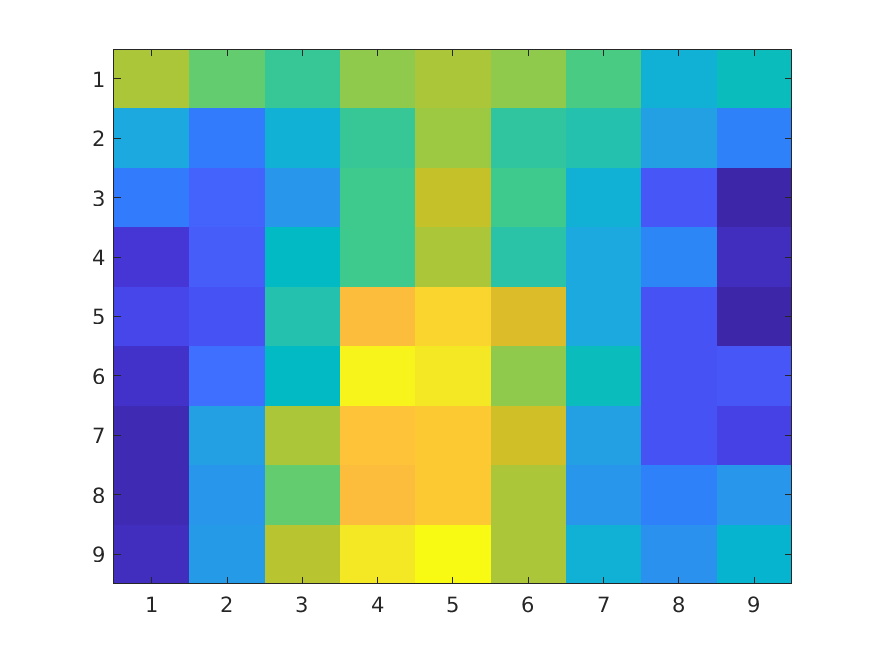
\includegraphics[width=0.2\linewidth]{images/Fig_weights_16.png}
\\
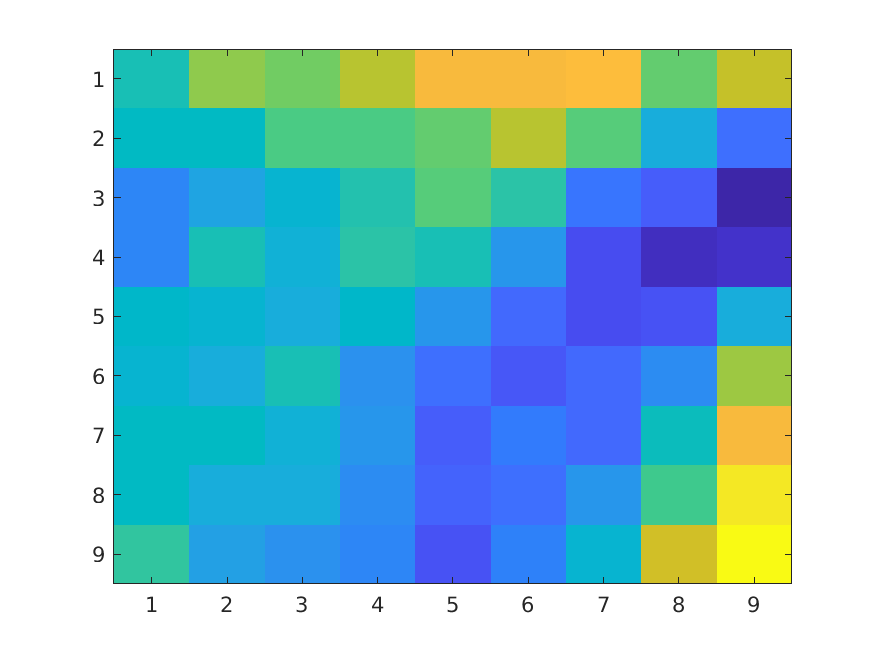
\includegraphics[width=0.2\linewidth]{images/Fig_weights_17.png}
&
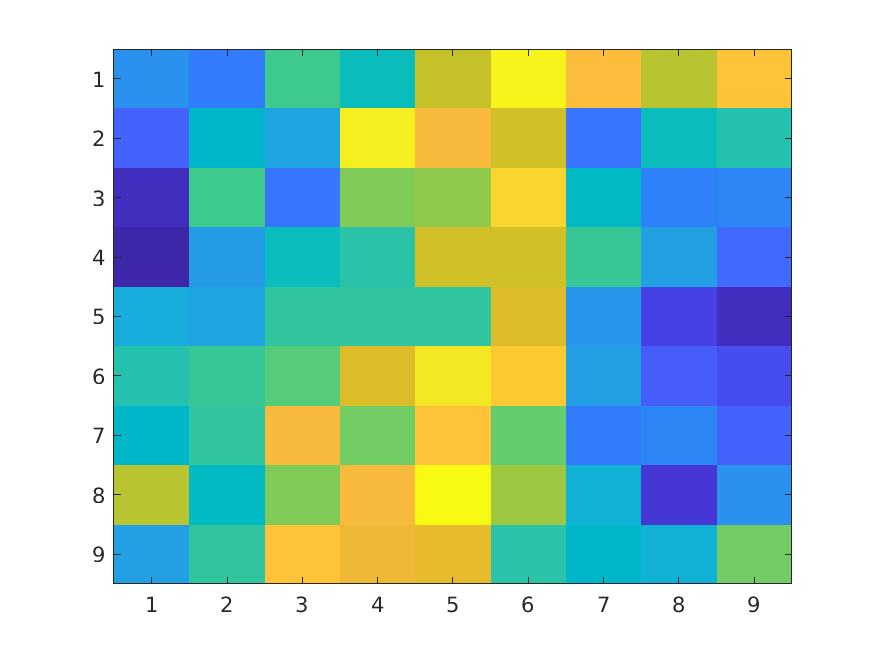
\includegraphics[width=0.2\linewidth]{images/Fig_weights_18.png}
&
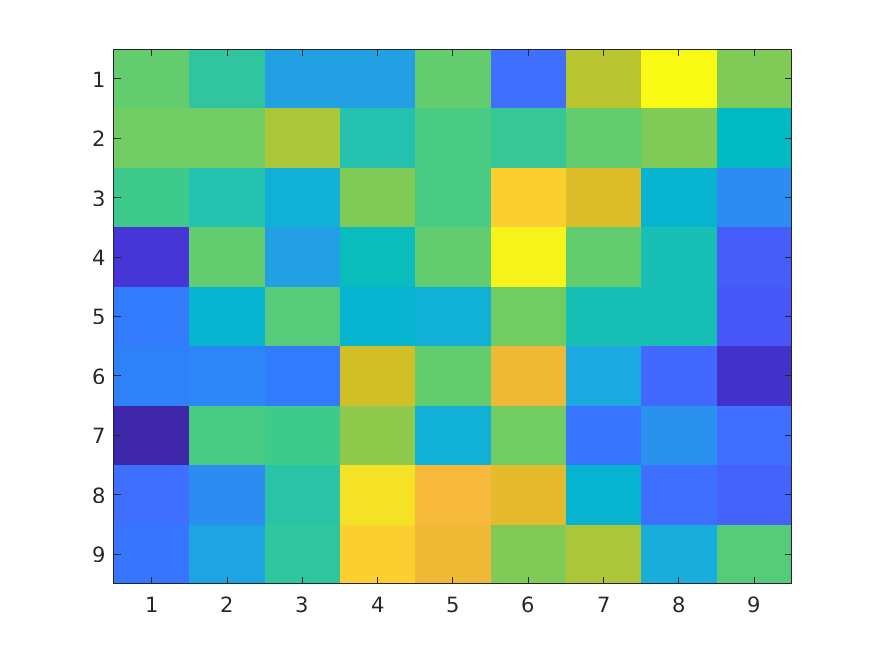
\includegraphics[width=0.2\linewidth]{images/Fig_weights_19.png}
&
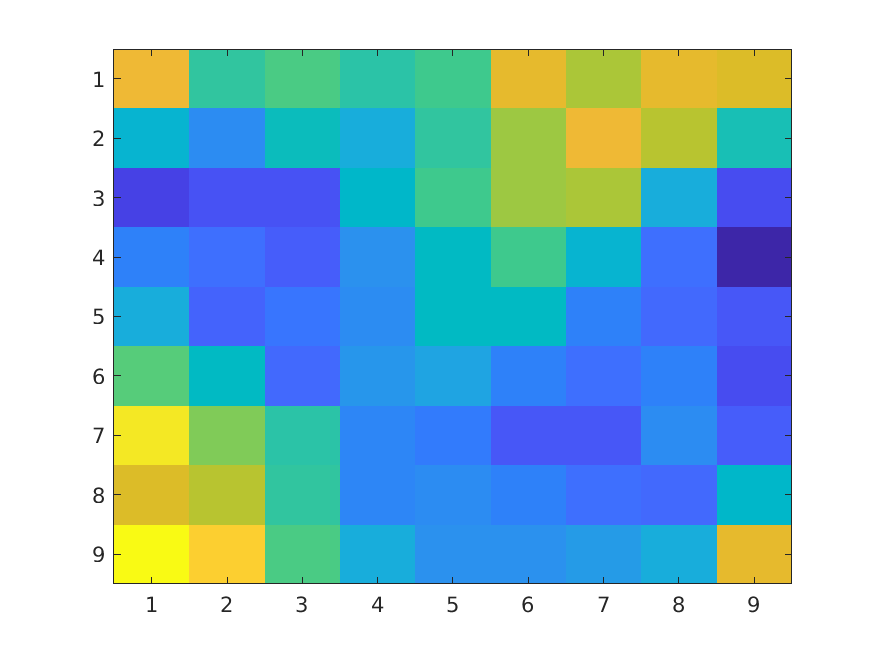
\includegraphics[width=0.2\linewidth]{images/Fig_weights_20.png}
\end{tabular}
\end{figure}

\newpage
The corresponding gray scale visualisation is given below :
\begin{figure}[H]
\centering
\begin{tabular}{cccc}
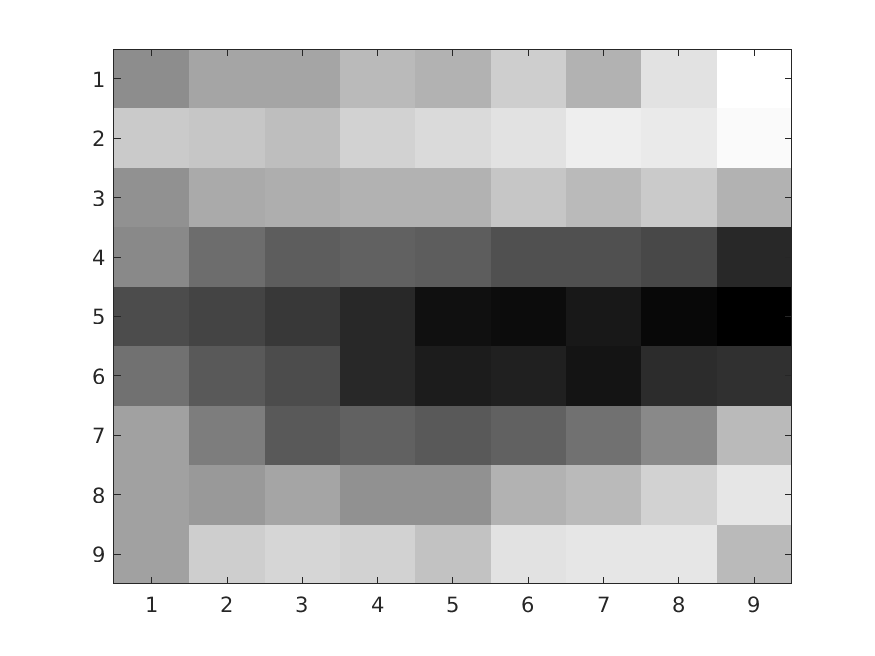
\includegraphics[width=0.2\linewidth]{images/Fig_grey_1.png}
&
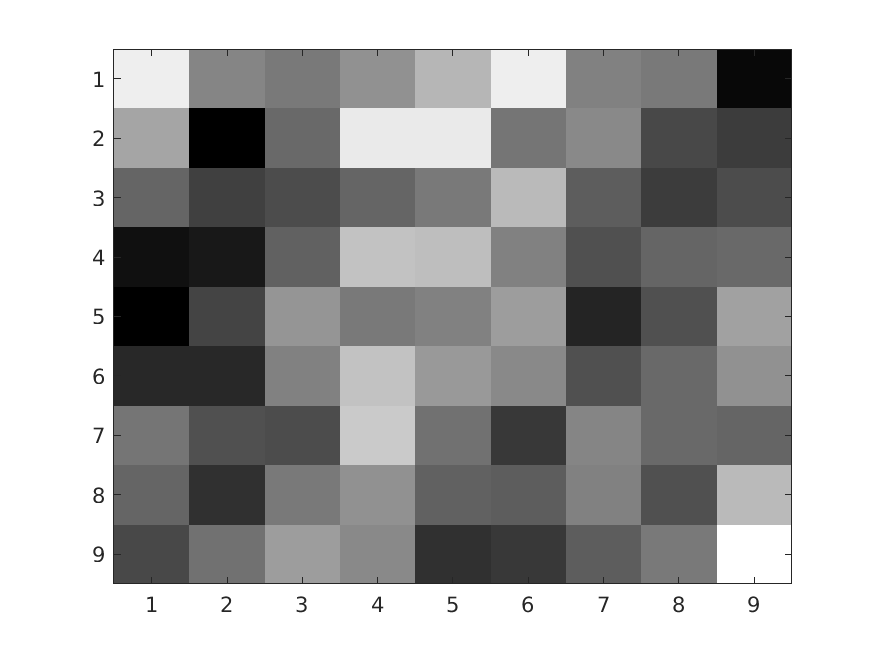
\includegraphics[width=0.2\linewidth]{images/Fig_grey_2.png}
&
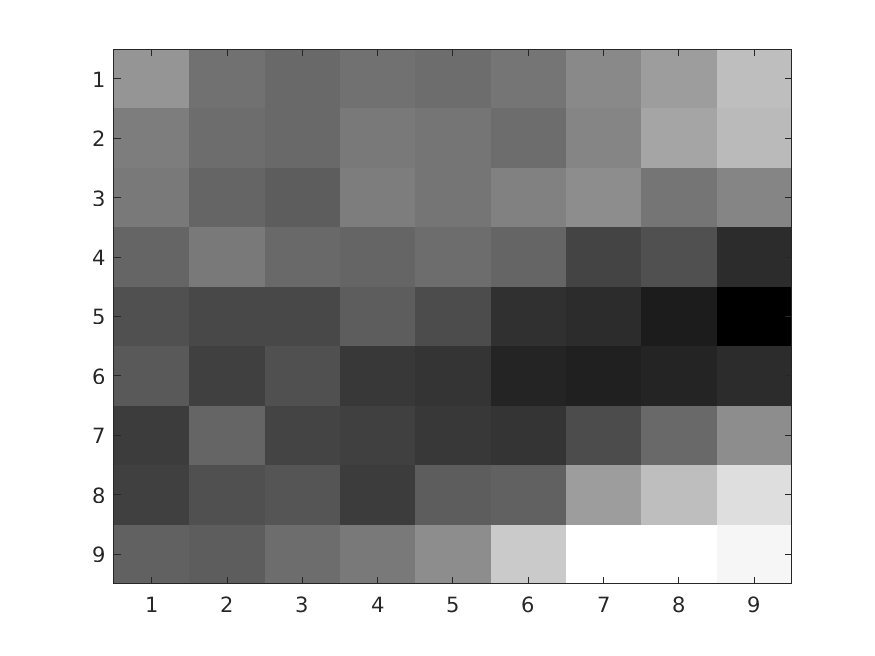
\includegraphics[width=0.2\linewidth]{images/Fig_grey_3.png}
&
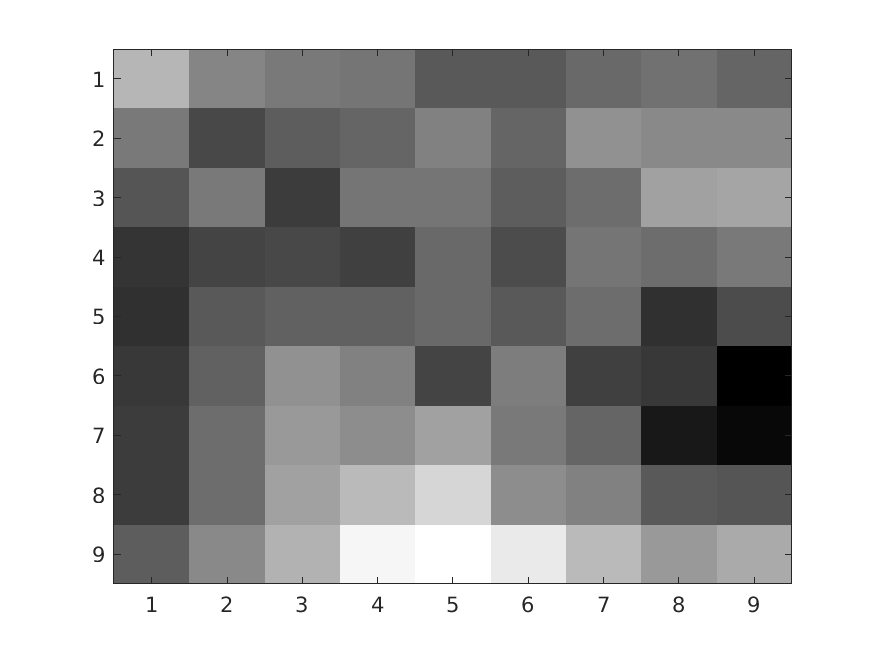
\includegraphics[width=0.2\linewidth]{images/Fig_grey_4.png}
\\
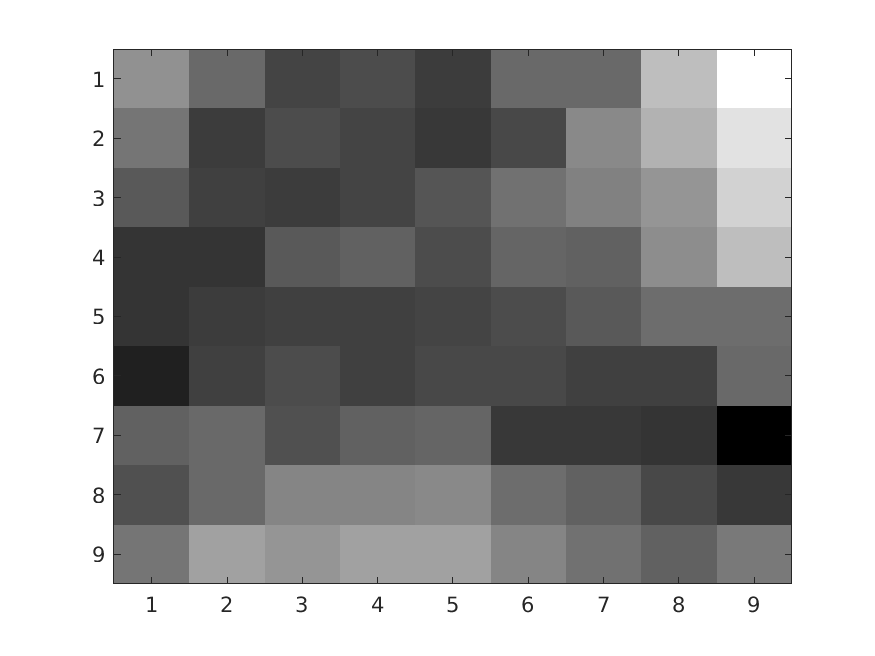
\includegraphics[width=0.2\linewidth]{images/Fig_grey_5.png}
&
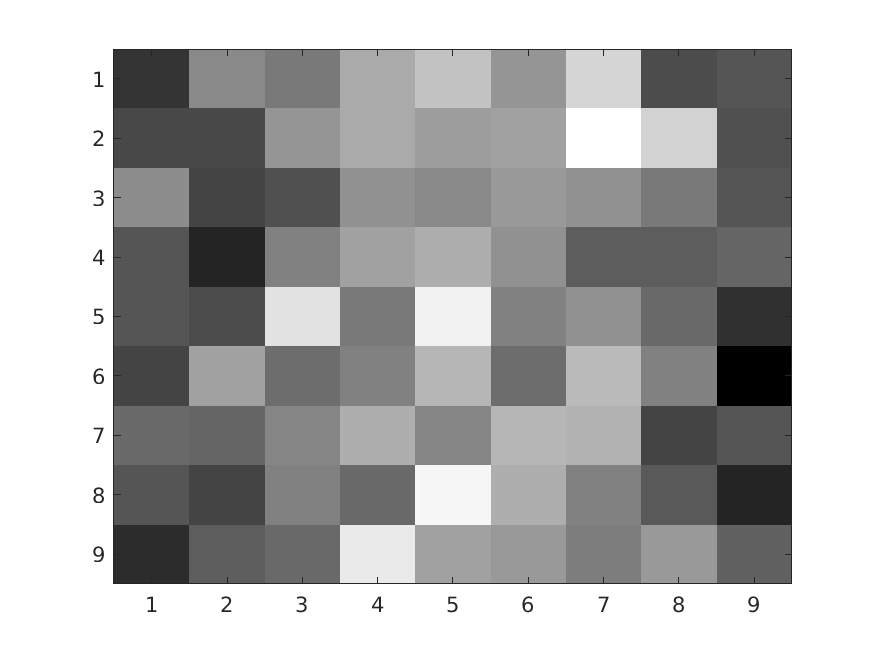
\includegraphics[width=0.2\linewidth]{images/Fig_grey_6.png}
&
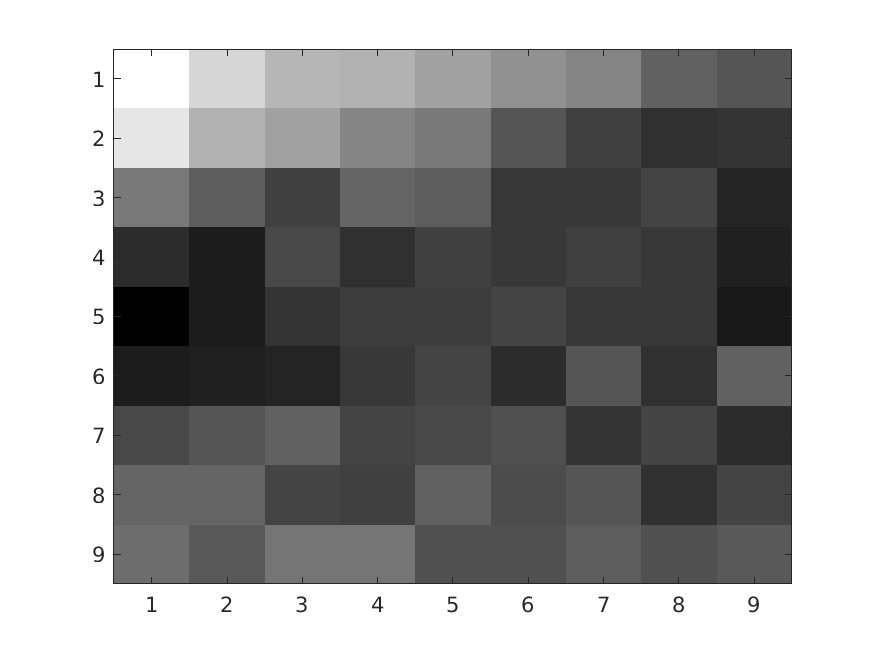
\includegraphics[width=0.2\linewidth]{images/Fig_grey_7.png}
&
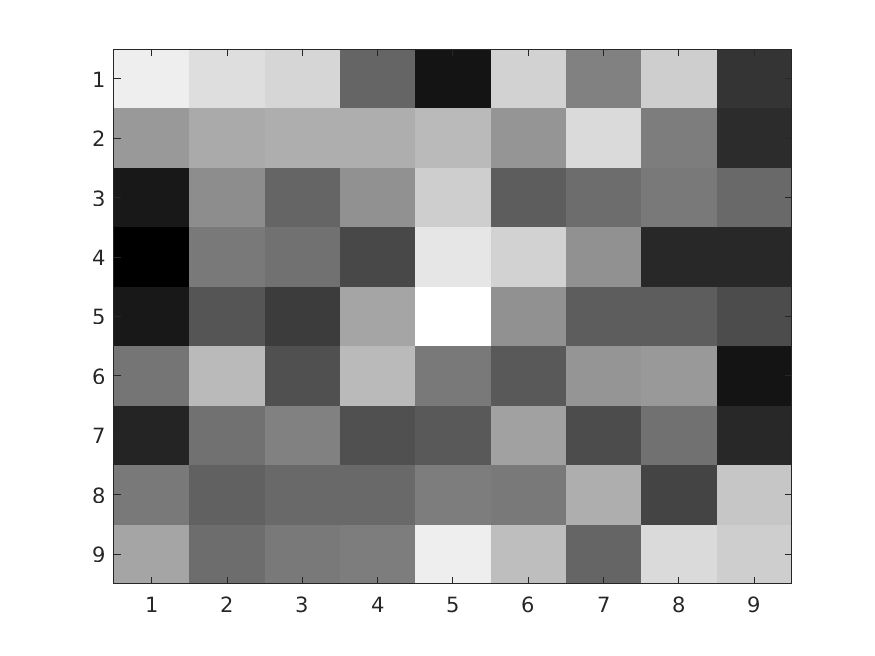
\includegraphics[width=0.2\linewidth]{images/Fig_grey_8.png}
\\
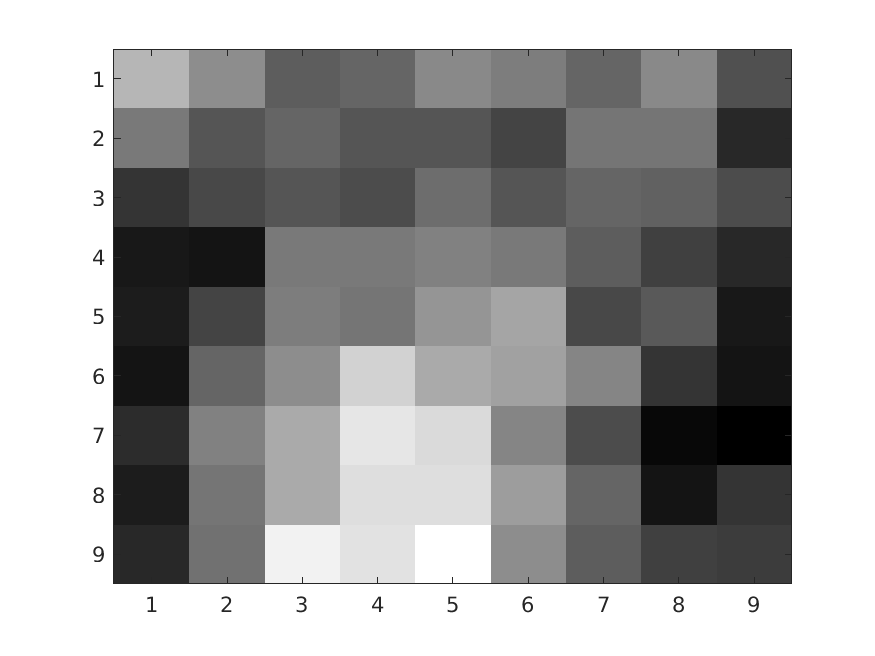
\includegraphics[width=0.2\linewidth]{images/Fig_grey_9.png}
&
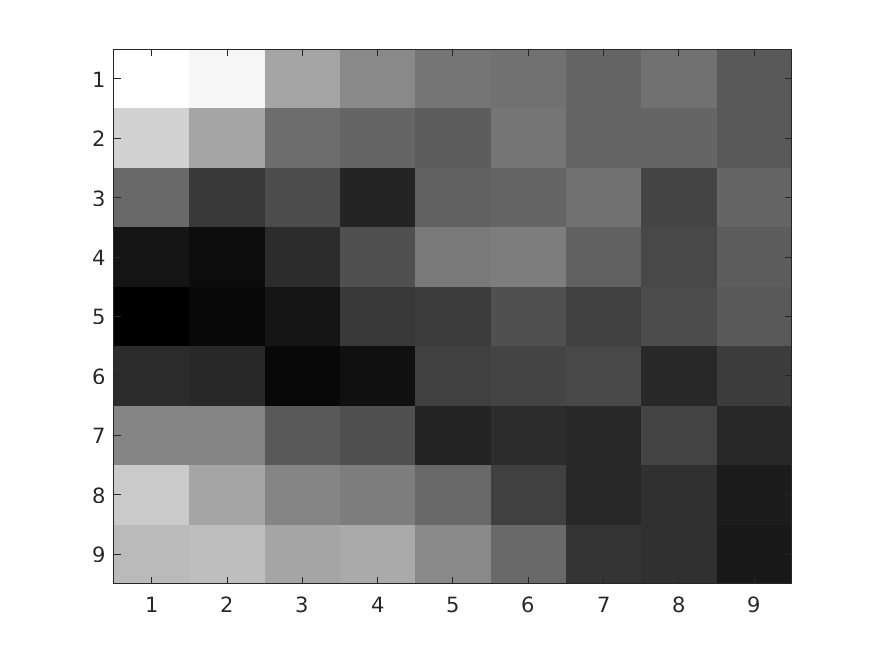
\includegraphics[width=0.2\linewidth]{images/Fig_grey_10.png}
&
\includegraphics[width=0.2\linewidth]{images/Fig_grey_11.png}
&
\includegraphics[width=0.2\linewidth]{images/Fig_grey_12.png}
\\
\includegraphics[width=0.2\linewidth]{images/Fig_grey_13.png}
&
\includegraphics[width=0.2\linewidth]{images/Fig_grey_14.png}
&
\includegraphics[width=0.2\linewidth]{images/Fig_grey_15.png}
&
\includegraphics[width=0.2\linewidth]{images/Fig_grey_16.png}
\\
\includegraphics[width=0.2\linewidth]{images/Fig_grey_17.png}
&
\includegraphics[width=0.2\linewidth]{images/Fig_grey_18.png}
&
\includegraphics[width=0.2\linewidth]{images/Fig_grey_19.png}
&
\includegraphics[width=0.2\linewidth]{images/Fig_grey_20.png}
\end{tabular}
\end{figure}



\textbf{NOTE : }The python file for loading \textbf{\textit{CNN$\_$Network}} and plotting the filters has been named \textbf{\textit{"visualise.m"}}\\\\

If we compare the arrangement to a matrix with 5 rows and 4 columns indexed from [1,1] to [5,4], the we can see that :
\begin{itemize}
    \item Filter [1,1] responds to a horizontal lines
    \item Filter [4,4] responds to vertical lines
    \item Filter [1,3], [4,1] and [5,1] respond to lines that are slanting right
    \item Filter [3,2] and [4,2] responds to lines slanting left
    \item Filter [2,1], [3,4] and [5,4] may respond to curvy edges
\end{itemize}

%%%%%%%%%%%%%%%%%%%%%%%%%%%%%%%%%%%%%%%%%%%%%%%%%%%%%%%%%%%%%%%%%
\newpage
\section{Question 3}
While doing Hyperparameter tuning using 3 different values each for \textit{No. of Epochs}, \textit{No. of Filters} and \textit{Filter Dimension} by training using initial 1000 training images, we obtain the following results :
\begin{table}[H]
  \begin{center}
    \begin{tabular}{| c | c | c | c | c |} 
    \hline
      \textbf{No. of Epochs} & \textbf{No. of Filters} & \textbf{Filter Dimension} & \textbf{Accuracy} & \textbf{Training time}\\
      \hline
      5 & 16 & 3 & 77.29 & 17.95s\\
      \hline
      5 & 16 & 5 & 80.45 & 15.02s\\
      \hline
      5 & 16 & 11 & 85.63 & 9.41s\\
      \hline
      5 & 25 & 3 & 75.85 & 28.09s\\
      \hline
      5 & 25 & 5 & 78.22 & 23.73\\
      \hline
      5 & 25 & 11 & 87.97 & 17.19\\
      \hline
      5 & 36 & 3 & 75.06 & 39.39\\
      \hline
      5 & 36 & 5 & 68.95 & 33.63\\
      \hline
      5 & 36 & 11 & 86.22 & 20.53\\
      \hline %%%%%%%%%%%%%%%%%
      10 & 16 & 3 & 74.57 & 17.6s\\
      \hline
      10 & 16 & 5 & 74.9 & 15.28s\\
      \hline
      10 & 16 & 11 & 88.08 & 9.35\\
      \hline
      10 & 25 & 3 & 73.57 & 27.13s\\
      \hline
      10 & 25 & 5 & 74.61 & 23.41s\\
      \hline
      10 & 25 & 11 & 87.01 & 14.36s\\
      \hline
      10 & 36 & 3 & 72.45 & 38.73s\\
      \hline
      10 & 36 & 5 & 70.22 & 33.56s\\
      \hline
      10 & 36 & 11 & 84.86 & 20.46s\\
      \hline %%%%%%%%%%%%%%%%%%%
      20 & 16 & 3 & 74.7 &17.39s \\
      \hline
      20 & 16 & 5 & 78.12 & 15.21s\\
      \hline
      20 & 16 & 11 & 87.62 & 9.34s\\
      \hline
      20 & 25 & 3 & 73.48 & 27.03s\\
      \hline
      20 & 25 & 5 & 73.14 & 23.57s\\
      \hline
      20 & 25 & 11 & 86.97 & 14.36s\\
      \hline
      20 & 36 & 3 & 72.7 & 38.78s\\
      \hline
      20 & 36 & 5 & 69.25 & 33.40s\\
      \hline
      20 & 36 & 11 & 83.92 & 20.5s \\
      \hline
    \end{tabular}
  \end{center}
\end{table}

To get a better analysis : Red, Green and Blue dots correspond to Filter sizes 16, 25 and 36 respectively.
%-------------------------------------------------
\subsection{For No. of epochs = 5}
\begin{figure}[H]
\centering
\begin{tabular}{cc}
\includegraphics[width=0.5\linewidth]{images/e5a1.png}
&
\includegraphics[width=0.5\linewidth]{images/e5a2.png}
\\
\includegraphics[width=0.5\linewidth]{images/e5t1.png}
&
\includegraphics[width=0.5\linewidth]{images/e5t2.png}
\end{tabular}
\end{figure}

%-------------------------------------------------
\subsection{For No. of epochs = 10}
\begin{figure}[H]
\centering
\begin{tabular}{cc}
\includegraphics[width=0.5\linewidth]{images/e10a1.png}
&
\includegraphics[width=0.5\linewidth]{images/e10a2.png}
\\
\includegraphics[width=0.5\linewidth]{images/e10t1.png}
&
\includegraphics[width=0.5\linewidth]{images/e10t2.png}
\end{tabular}
\end{figure}

%-------------------------------------------------
\subsection{For No. of epochs = 20}
\begin{figure}[H]
\centering
\begin{tabular}{cc}
\includegraphics[width=0.5\linewidth]{images/e20a1.png}
&
\includegraphics[width=0.5\linewidth]{images/e20a2.png}
\\
\includegraphics[width=0.5\linewidth]{images/e20t1.png}
&
\includegraphics[width=0.5\linewidth]{images/e20t2.png}
\end{tabular}
\end{figure}

\newpage
\subsection{Observations}
As can be seen from the above plots :
\begin{itemize}
    \item Accuracy generally decreases as the number of filters increases, given a constant no. of training epochs. This could probably be due to insufficient training of larger number of weights compared to when there are smaller no. of weights.
    \item Accuracy generally increases as the dimension of filters increases, given a constant no. of training epochs. This could probably be because more spatial information is captured while using a larger filter in place of a smaller filter. If this is was a deeper network, then the larger spatial dependence could have been captured in deeper layers. But since this is a shallow network with just one convolutional layer, larger filter helps capture spatial dependencies between the pixels of the image that could aid in better classification results.
    \item Training time generally increases as the number of filters increases, given a constant no. of training epochs. This is because the number of weights increases and hence the number of updates also increases and hence the training time increases with the amount of additional computation required (especially in the last fully connected layer).
    \item Training time generally decreases as the filter size increases, given constant no. of epochs and no. of filters. This is because the no. of neurons in the fully connected layer reduces due to reduction in the output image size after convolution. Since majority of neurons are present in the fully connected layer (Convolutional layer has weight sharing since the same filter is used over the entire image), the effective amount of computation required reduces and hence training time reduces.
\end{itemize}

\textbf{Note : }The code for plotting has been named \textbf{"plot.py"}\\\\
\textbf{Note : }The code for generating the results for the hyperparameter tuning has been named \textbf{\textit{Traincnn$\_$loop.m}} and for malual tuning, use \textit{Traincnn$\_$tuning.m}
\end{document} % NOTHING AFTER THIS LINE IS PART OF THE DOCUMENT
 ______ ______ ______ ______ ______ ______ ______ 
|______|______|______|______|______|______|______|
				  _____  ____  
				 / ____|/ __ \ 
				| |  __  |  | |
				| | |_ | |  | |
				| |__| | |__| |
				 \_____|\____/ 
 
 _    _  ____  _____  _   _ ______ _______ _____ _ 
| |  | |/ __ \|  __ \| \ | |  ____|__   __/ ____| |
| |__| | |  | | |__) |  \| | |__     | | | (___ | |
|  __  | |  | |  _  /| . ` |  __|    | |  \___ \| |
| |  | | |__| | | \ \| |\  | |____   | |  ____) |_|
|_|  |_|\____/|_|  \_\_| \_|______|  |_| |_____/(_)

 ______ ______ ______ ______ ______ ______ ______ 
|______|______|______|______|______|______|______|